\documentclass[aspectratio=169]{beamer}
\usepackage[utf8]{inputenc}
\usepackage[T1]{fontenc}
\usepackage{booktabs}
\usepackage{colortbl}
\usepackage{graphicx}
\usepackage{xcolor}
\usepackage{tikz}
\usetikzlibrary{positioning,arrows.meta,shapes.geometric}
\usepackage{pgfplots}
\pgfplotsset{compat=1.18}
\usepackage{amsmath}
\usepackage{tcolorbox}
\tcbuselibrary{skins}

\definecolor{cdark}{HTML}{0D2137}
\definecolor{cmid}{HTML}{065A82}
\definecolor{cteal}{HTML}{02C39A}
\definecolor{clight}{HTML}{E8F4F8}
\definecolor{ctext}{HTML}{1A2E40}
\definecolor{cmuted}{HTML}{607D8B}
\definecolor{cwarn}{HTML}{F4A261}
\definecolor{cgap}{HTML}{E63946}
\definecolor{caccent}{HTML}{A0BFD0}
\definecolor{cbg2}{HTML}{028090}

\usetheme{default}
\usecolortheme{default}
\setbeamertemplate{navigation symbols}{}
\usefonttheme{professionalfonts}
\setbeamerfont{frametitle}{size=\large,series=\bfseries}
\setbeamercolor{frametitle}{fg=cdark,bg=white}
\setbeamercolor{normal text}{fg=ctext}
\setbeamercolor{background canvas}{bg=white}
\setbeamercolor{item}{fg=cteal}

\addtobeamertemplate{frametitle}{}{%
  \vspace{-4pt}\textcolor{cteal}{\hrule height 1.5pt}\vspace{3pt}}

\setbeamertemplate{footline}{%
  \leavevmode\hbox{%
    \begin{beamercolorbox}[wd=0.85\paperwidth,ht=2.2ex,dp=1ex,leftskip=4pt]{normal text}%
      \tiny\color{cmuted}An Pham \textbar{} LIRMM--ADVANSE \textbar{} Luc \& Reda%
    \end{beamercolorbox}%
    \begin{beamercolorbox}[wd=0.15\paperwidth,ht=2.2ex,dp=1ex,right,rightskip=6pt]{normal text}%
      \scriptsize\color{cmuted}\insertframenumber/\inserttotalframenumber%
    \end{beamercolorbox}}}

\setbeamertemplate{itemize item}{\color{cteal}\textbullet}
\setbeamertemplate{itemize subitem}{\color{cmid}--}
\setlength{\leftmargini}{1em}

\tikzset{
  flowbox/.style={rounded corners, draw=cmid, fill=clight, align=center,
    minimum height=0.9cm, text width=2.6cm, font=\footnotesize},
  flowarrow/.style={-Latex, thick, color=cmid}
}

\title{\textbf{Mixed-Length Shapelets to KMeans}}
\subtitle{Pipeline and Explanation Stage}
\author{An Pham}
\institute{LIRMM--ADVANSE, Universit\'e de Montpellier}
\date{May 27, 2026}

\begin{document}

% --- Slide 1 ---
{\setbeamercolor{background canvas}{bg=cdark}
\begin{frame}[plain]
\begin{tikzpicture}[remember picture,overlay]
  \fill[cteal](current page.north west)rectangle([xshift=6pt]current page.south west);
\end{tikzpicture}
\vspace{1.1cm}
{\color{white}\huge\bfseries Mixed-Length Shapelets to KMeans}\\[5pt]
{\color{cteal}\large\itshape Pipeline and Explanation Stage}\\[8pt]
{\color{caccent}\small Explainable Clustering for Spatio-Temporal Data}\\[0.6cm]
{\color{cmid}\rule{5.6cm}{0.8pt}}\\[5pt]
{\color{caccent}\footnotesize\textbf{An Pham}\quad|\quad LIRMM--ADVANSE\quad|\quad Supervisors: Luc \& Reda}\\[2pt]
{\color{caccent}\footnotesize May 27, 2026}
\end{frame}}

% --- Slide 2 ---
\begin{frame}{What This Deck Explains}
\begin{columns}[T,onlytextwidth]
  \column{0.55\textwidth}
  \begin{itemize}\footnotesize\setlength\itemsep{4pt}
    \item How mixed-length shapelets are sampled and selected.
    \item How distances to shapelets become a fixed-width feature vector.
    \item How KMeans is selected and fit on the shapelet-distance matrix.
    \item How explanations are derived from surrogate + SHAP + abductive edits.
  \end{itemize}
  \column{0.45\textwidth}
  \begin{tcolorbox}[enhanced,boxrule=1pt,arc=2pt,colback=clight,colframe=cmid]
    \footnotesize\textbf{Code anchors}\\[2pt]
    \tiny
    \texttt{scripts/research/}\\
    \texttt{shapelet\_stability.py}\\
    \texttt{scripts/notebooks/}\\
    \texttt{shapelets\_ecg200.ipynb}\\
    \texttt{shapelets\_ecg5000.ipynb}\\
    \texttt{shapelets\_roma\_taxi.ipynb}
  \end{tcolorbox}
\end{columns}
\end{frame}

% --- Slide 3 ---
\begin{frame}{Mixed-Length Shapelets: Visual Intuition}
\begin{columns}[T,onlytextwidth]
  \column{0.6\textwidth}
  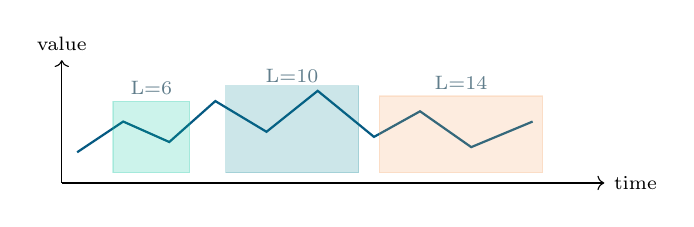
\begin{tikzpicture}[scale=0.65]
    \draw[->] (0,0) -- (10.6,0) node[right]{\scriptsize time};
    \draw[->] (0,0) -- (0,2.4) node[above]{\scriptsize value};
    \draw[thick,cmid] plot coordinates {(0.3,0.6) (1.2,1.2) (2.1,0.8) (3.0,1.6) (4.0,1.0) (5.0,1.8) (6.1,0.9) (7.0,1.4) (8.0,0.7) (9.2,1.2)};

    \draw[fill=cteal,opacity=0.2,draw=cteal] (1.0,0.2) rectangle (2.5,1.6);
    \node[cmuted] at (1.75,1.85) {\scriptsize L=6};

    \draw[fill=cbg2,opacity=0.2,draw=cbg2] (3.2,0.2) rectangle (5.8,1.9);
    \node[cmuted] at (4.5,2.1) {\scriptsize L=10};

    \draw[fill=cwarn,opacity=0.2,draw=cwarn] (6.2,0.2) rectangle (9.4,1.7);
    \node[cmuted] at (7.8,1.95) {\scriptsize L=14};
  \end{tikzpicture}
  \column{0.4\textwidth}
  \begin{itemize}\footnotesize\setlength\itemsep{4pt}
    \item Candidate shapelets are sampled from multiple lengths.
    \item Mixed lengths capture short and long motifs in one dictionary.
    \item Each shapelet becomes one feature after distance transform.
  \end{itemize}
\end{columns}
\end{frame}

% --- Slide 4 ---
\begin{frame}{Pipeline Overview (Data Flow)}
\begin{center}
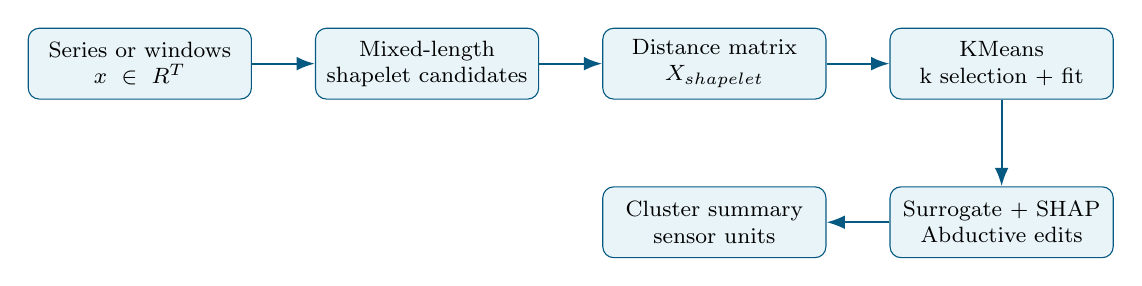
\begin{tikzpicture}[node distance=1.1cm and 0.8cm]
  \node[flowbox] (raw) {Series or windows\\$x \in \mathbb{R}^{T}$};
  \node[flowbox, right=of raw] (shapelets) {Mixed-length\\shapelet candidates};
  \node[flowbox, right=of shapelets] (dist) {Distance matrix\\$X_{shapelet}$};
  \node[flowbox, right=of dist] (kmeans) {KMeans\\k selection + fit};
  \node[flowbox, below=of kmeans] (explain) {Surrogate + SHAP\\Abductive edits};
  \node[flowbox, left=of explain] (report) {Cluster summary\\sensor units};

  \draw[flowarrow] (raw) -- (shapelets);
  \draw[flowarrow] (shapelets) -- (dist);
  \draw[flowarrow] (dist) -- (kmeans);
  \draw[flowarrow] (kmeans) -- (explain);
  \draw[flowarrow] (explain) -- (report);
\end{tikzpicture}
\end{center}
\vspace{4pt}
{\scriptsize\itshape Mixed-length sampling gives one dictionary; distances make it fixed-width.\\
KMeans runs on that matrix; explanations follow.}
\end{frame}

% --- Slide 5 ---
\begin{frame}{Step 1: Build a Mixed-Length Dictionary}
\begin{columns}[T,onlytextwidth]
  \column{0.6\textwidth}
  \begin{itemize}\footnotesize\setlength\itemsep{4pt}
    \item Input: $x \in \mathbb{R}^{N \times T}$, length list (e.g., \texttt{(5, 10, 15, 20)}).
    \item For each candidate, randomly choose length, series, and start index.
    \item Code: \texttt{extract\_random\_shapelets} in \texttt{shapelet\_stability.py}.
  \end{itemize}
  \column{0.4\textwidth}
  \begin{tcolorbox}[enhanced,boxrule=1pt,arc=2pt,colback=clight,colframe=cmid]
    \ttfamily\footnotesize
    for cand in 1..n\_candidates:\\
    \ \ L = choice(lengths)\\
    \ \ row = random series\\
    \ \ start = random index\\
    \ \ s = x[row, start:start+L]
  \end{tcolorbox}
\end{columns}
\vspace{4pt}
{\scriptsize\color{cmuted}Mixed lengths are explicit in the \texttt{lengths} list and sampled per candidate.}
\end{frame}

% --- Slide 6 ---
\begin{frame}{Step 2: Shapelet-Distance Feature Matrix}
\begin{columns}[T,onlytextwidth]
  \column{0.55\textwidth}
  \begin{itemize}\footnotesize\setlength\itemsep{4pt}
    \item Each shapelet yields one feature: distance from a series to that shapelet.
    \item Implementation: \texttt{min\_distance\_to\_shapelet} + \texttt{compute\_shapelet\_distances}.
    \item Standardize the distance matrix before KMeans.
  \end{itemize}
  \column{0.45\textwidth}
  \begin{block}{Distance mapping}
  \vspace{-6pt}
  \[
  \phi_j(x) = \min_{t} \lVert x[t:t+L_j] - s_j \rVert_2
  \]
  \[
  X_{shapelet} \in \mathbb{R}^{N \times m}
  \]
  \end{block}
\end{columns}
\vspace{4pt}
{\scriptsize\itshape Mixed-length shapelets still produce a fixed-width matrix because each shapelet contributes one column.}
\end{frame}

% --- Slide 7 ---
\begin{frame}{Step 3: KMeans Selection and Clustering}
\begin{columns}[T,onlytextwidth]
  \column{0.6\textwidth}
  \begin{itemize}\footnotesize\setlength\itemsep{4pt}
    \item Evaluate k on shapelet features with multiple seeds.
    \item Metrics: silhouette and stability ARI across seeds.
    \item Composite score: \texttt{silhouette + 0.5 * stability\_ari}.
    \item Code: \texttt{search\_best\_k} + final \texttt{KMeans} fit.
  \end{itemize}
  \column{0.4\textwidth}
  \begin{tcolorbox}[enhanced,boxrule=1pt,arc=2pt,colback=clight,colframe=cmid]
    \ttfamily\footnotesize
    for k in k\_grid:\\
    \ \ labels = KMeans(k).fit\_predict(X)\\
    \ \ sil = silhouette(labels)\\
    \ \ stability = mean(ARI)\\
    \ score = sil + 0.5*stability
  \end{tcolorbox}
\end{columns}
\end{frame}

% --- Slide 8 ---
\begin{frame}{Step 4: Explanation Stage (Transparent Outputs)}
\begin{columns}[T,onlytextwidth]
  \column{0.52\textwidth}
  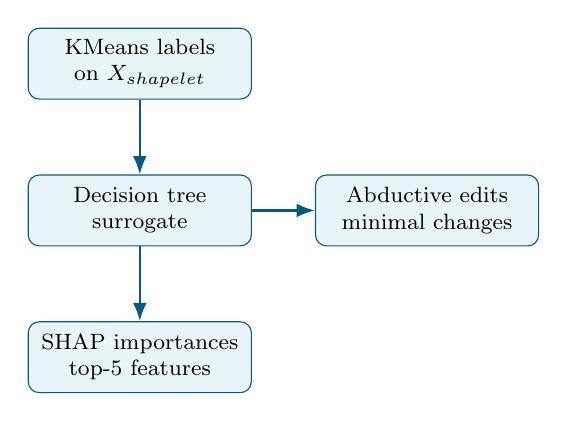
\begin{tikzpicture}[node distance=0.95cm and 0.8cm]
    \node[flowbox] (labels) {KMeans labels\\on $X_{shapelet}$};
    \node[flowbox, below=of labels] (tree) {Decision tree\\surrogate};
    \node[flowbox, below=of tree] (shap) {SHAP importances\\top-5 features};
    \node[flowbox, right=of tree] (abduct) {Abductive edits\\minimal changes};

    \draw[flowarrow] (labels) -- (tree);
    \draw[flowarrow] (tree) -- (shap);
    \draw[flowarrow] (tree) -- (abduct);
  \end{tikzpicture}
  \column{0.48\textwidth}
  \begin{itemize}\footnotesize\setlength\itemsep{4pt}
    \item Surrogate: \texttt{DecisionTreeClassifier} on shapelet features.
    \item Fidelity: cross-validated accuracy vs KMeans labels.
    \item Stability: top-5 feature overlap across seeds.
    \item Abductive: minimal feature edits that flip cluster.
  \end{itemize}
\end{columns}
\end{frame}

% --- Slide 9 ---
\begin{frame}{Supervisor-Ready Outputs}
\begin{itemize}\footnotesize\setlength\itemsep{4pt}
  \item Slide deck: \texttt{docs/slides/2026-05-27/}\\
  \texttt{shapelets\_mixed\_length\_kmeans.pdf}.
  \item Pipeline notes: \texttt{docs/SHAPELETS\_WORK\_NOTES.md}.
  \item Core implementation: \texttt{scripts/research/}\\
  \texttt{shapelet\_stability.py}.
  \item Dataset-specific notebooks for figures and runs: \texttt{shapelets\_ecg200}, \texttt{shapelets\_ecg5000}, \texttt{shapelets\_roma\_taxi}.
\end{itemize}
\vspace{6pt}
{\scriptsize\itshape Use the pipeline diagram and Step 2/3 slides to explain the mixed-length to KMeans transition clearly.}
\end{frame}

\end{document}
